\RequirePackage{plautopatch}
\documentclass[uplatex,dvipdfmx,titlepage,a4j]{jsarticle}
\usepackage{amsmath,amssymb}
\usepackage{graphicx}
\usepackage[yen]{okuverb}
\usepackage{siunitx}
\usepackage{askmaps}
\usepackage{subfigure}

\makeatletter
\newcommand{\tblcaption}[2]{\def\@captype{table}\caption{#1}\label{tab: #2}}
\makeatother

\begin{document}

\section{Draw.io のやつ}

% fimg [enter] diagram [enter] [enter] diagram [enter]
\begin{figure}[h]
  \centering
  \includegraphics[width=3cm]{diagram.pdf}
  \caption{diagram} \label{fig: diagram}
\end{figure}

\section{table 自動生成}

% data/table-1/table.tex から直コピーした
\begin{table}[hbtp]
  \caption{表のデモ} \label{tab: 表のデモ}
  \centering
  \renewcommand{\arraystretch}{0.7}
  \begin{tabular}{ccc}

\hline
a & b & c \\
\hline
1 & 2 & 3 \\
2 & 3 & 4 \\
    \hline
  \end{tabular}
\end{table}

%

\section{gnuplot 連携}

\begin{figure}[h]
  \centering
  \includegraphics[width=12cm]{chart-1}
  \caption{chart-1} \label{fig: chart-1}
\end{figure}

\section{png への画像変換}

\begin{figure}[h]
  \centering

  \begin{minipage}{0.3\textwidth}
    \centering
    \includegraphics[width=3cm]{bmp.png}
    \caption{BMP} \label{fig: bmp.png}
  \end{minipage}

  \begin{minipage}{0.3\textwidth}
    \centering
    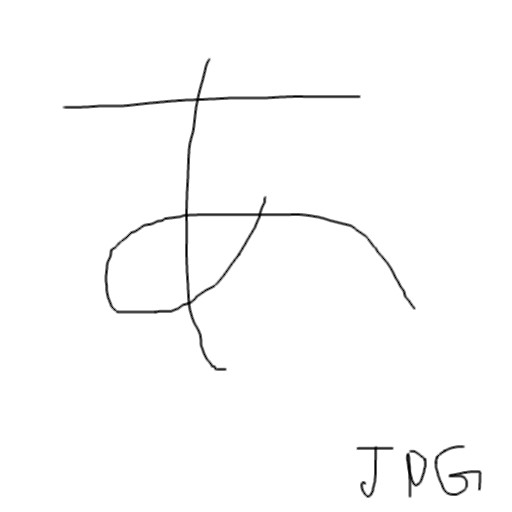
\includegraphics[width=3cm]{jpg.png}
    \caption{JPG} \label{fig: jpg.png}
  \end{minipage}

  \begin{minipage}{0.3\textwidth}
    \centering
    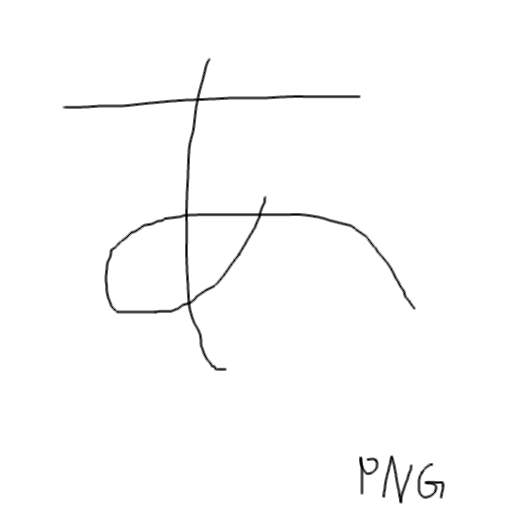
\includegraphics[width=3cm]{png.png}
    \caption{PNG} \label{fig: png.png}
  \end{minipage}

\end{figure}


\begin{thebibliography}{99}
  \bibitem{citelabel1}{
    % 参考文献
  }
\end{thebibliography}

\end{document}